\documentclass[letterpaper, 10 pt, conference]{sty/ieeeconf}

\IEEEoverridecommandlockouts

\overrideIEEEmargins

\usepackage{graphics}
\usepackage{epsfig}
\usepackage{amsmath}
\usepackage{amssymb}
\usepackage{txfonts}
\usepackage{tikz}
\usepackage{sty/tkz-base}
\usepackage[T1]{fontenc}

\usetikzlibrary{shapes,decorations,shadows}
\usetikzlibrary{decorations.pathmorphing}
\usetikzlibrary{decorations.shapes}
\usetikzlibrary{fadings}
\usetikzlibrary{patterns}
\usetikzlibrary{calc}
\usetikzlibrary{decorations.text}
\usetikzlibrary{decorations.footprints}
\usetikzlibrary{decorations.fractals}
\usetikzlibrary{shapes.gates.logic.IEC}
\usetikzlibrary{shapes.gates.logic.US}
\usetikzlibrary{fit,chains}
\usetikzlibrary{positioning}
\usepgflibrary{shapes}
\usetikzlibrary{scopes}
\usetikzlibrary{arrows}
\usetikzlibrary{backgrounds}
\tikzset{latent/.style={circle,fill=white,draw=black,inner sep=1pt, 
minimum size=20pt, font=\fontsize{10}{10}\selectfont},
obs/.style={latent,fill=gray!25},
const/.style={rectangle, inner sep=0pt},
factor/.style={rectangle, fill=gray!25,minimum size=15pt, inner sep=1pt,draw=black},
>={triangle 45}}

\DeclareMathOperator*{\argmax}{arg\,max}
\DeclareMathOperator*{\argmin}{arg\,min}

\begin{document}

\title{\LARGE \bf
Curb Detection for a Pedestrian Robot in Urban Environments
}

\author{
\authorblockN{
J\'{e}r\^{o}me Maye,
Ralf Kaestner,
and Roland Siegwart}
\authorblockA{
Autonomous Systems Lab, ETH Zurich, Switzerland\\
email: \{jerome.maye, ralf.kaestner, roland.siegwart\}@mavt.ethz.ch}
}

\maketitle

\begin{abstract}
This paper presents a novel ...

\end{abstract}

\section{Introduction}
CONTEXT OF THE PAPER.

SUMMARY OF THE PAPER.

CONTRIBUTIONS.

The rest of the paper is organized as follows. Section~\ref{sec:related}
summarizes the previous works related to ours. Section~\ref{sec:formulation}
introduces our Bayesian framework. Section~\ref{sec:exp} presents experimental
results. Section~\ref{sec:conc} outlines our conclusions and provides some
insights for future work.


\section{Related Work\label{sec:related}}
Some related works~\cite{oniga10polynomial,wijesoma04road,shin10drivable,pradeep08piece,yuan05dynamic,siegemund10curb}.


\section{Model\label{sec:model}}
In this Section, we establish the preliminary notations and introduce the
mathematical models that will be used throughout the paper.

\subsection{Measurements Representation}
A nodding laser range-finder produces scan measurements $\mathbf{s}_i=[r_i,
\theta_i,\psi_i]^\text{T}$ that are transformed into their corresponding
Cartesian 3D coordinates $\mathbf{p}_i=[x_i,y_i,z_i]^\text{T}$, where $r_i$ is
a range measurement, $\theta_i$ a pitch angle, and $\psi_i$ a bearing angle. The
sensing device has an error model which is typically a function of
$\mathbf{s}_i$, i.e. $e(\mathbf{s}_i)$. From a complete laser sweep, we obtain a
point cloud representation $\mathcal{P}=\{\mathbf{p}_1,\mathbf{p}_2,\dots,
\mathbf{p}_N\}$. $\mathcal{P}$ is finally projected onto a 2D grid $\mathcal{G}=
\{\mathcal{C}_1,\mathcal{C}_2,\dots,\mathcal{C}_M\}$, with cells $\mathcal{C}_i=
\{\mathbf{c}_i,h_i,l_i,\mathcal{I}_i\}$, where $\mathbf{c}_i$ is the center of
the cell, $h_i$ its height distribution, $l_i$ its label distribution, and
$\mathcal{I}_i=\{\mathbf{p}_j\mid\mathbf{p}_j\in\mathcal{P},j=\argmin_{j'}||
\mathbf{p}_{j'}-\mathbf{c}_i||,\mathbf{p}_{j_x}<\tau_{x_{max}},\mathbf{p}_{j_x}>
\tau_{x_{min}},\mathbf{p}_{j_y}<\tau_{y_{max}},\mathbf{p}_{j_y}>\tau_{y_{min}},
\mathbf{p}_{j_z}<\tau_{z_{max}},\mathbf{p}_{j_z}>\tau_{z_{min}}\}$. The
$\tau_{[x,y,z]_{[min,max]}}$ define boundaries for the 3D points.

The posterior height distribution is a normal distribution, such that $p(h_i)=
\mathcal{N}(h_i\mid\mu_{h_i},\sigma^2_{h_i},\mathcal{I}_i)$. $\mu_{h_i}$ is the
Maximum-Likelihood Estimate (MLE) for the cell mean computed with the values
$\mathbf{p}_{j_z}$, where $\mathbf{p}_j\in\mathcal{I}_i$. $\sigma^2_{h_i}$ is
the Maximum A-Posteriori (MAP) estimate for the cell variance. The prior
distribution for $\sigma^2_{h_i}$ is an inverse gamma distribution, where we
have inserted a simplified cell error model in the hyperparameters. The label
distribution is a discrete distribution over a set of labels
$\mathcal{L}=\{1,2,\dots,M\}$.

The grid $\mathcal{G}$ will also be referred to as a Digital Elevation Map (DEM)
in the rest of the paper. The choice of a DEM representation is mainly guided by
the final outcome of the algorithm, i.e. a traversability map for the planning
process. It is also convenient for defining Regions of Interest (ROI) in
$\mathcal{P}$ and for simplifying the subsequent computations. Whenever the
number of points that fall into a cell $\mathcal{C}_i$ is below a threshold,
i.e. $|\mathcal{I}_i|<\tau_{\mathcal{I}}$, it is flagged as invalid.

\subsection{Environment Model and Inference Task}
We assume a piecewise planar environment, i.e., the observed scene is composed
of a set of plane segments. Boundaries between plane segments define local
heights discontinuities that we shall term \emph{curbs} from now on. The major
inference task therefore boils down to discovering those plane segments. To this
end, we model the environment as a \emph{mixture of linear regressions}, which
yields the following generative process for the height values:

\begin{equation}
\label{eqn:mixture}
h_i\sim p(h_i\mid\Theta)=\sum_{k=1}^K\pi_k\mathcal{N}(h_i\mid
\mathbf{w}_k^\text{T}\boldsymbol{\phi}(\mathbf{c}_i),\sigma^2_k),
\end{equation}

where $\Theta=\{\boldsymbol{\pi},\mathbf{W},\boldsymbol{\sigma}^2\}$ is the set
of adaptive parameters, $\boldsymbol{\pi}=\{\pi_k\}$ are the mixture weights,
$\mathbf{W}=\{\mathbf{w}_k\}$ the regression coefficients,
$\boldsymbol{\sigma}^2=\{\sigma^2_k\}$ the regression variances, and
$\boldsymbol{\phi}(\mathbf{c}_i)=[1,\mathbf{c}_i]^\text{T}$ is the basis
function.

Similarly to Gaussian Mixture Models (GMM), one can resort to the popular
Expectation-Maximization (EM) algorithm~\cite{dempster77maximum} for estimating
the parameter set $\Theta$ given a set of observations
$\{\{h_i,\mathbf{c}_i\}\}_{i=1}^M$. The algorithm alternates between the
computation of \emph{responsibilities} $\gamma_{ik}$ given an old estimate
$\Theta^\text{old}$, and the computation of $\Theta^\text{new}$ given
$\Theta^\text{old}$ and $\gamma_{ik}$.

In order to determine the number of planes $k$ and the initial responsibilities,
we apply the algorithm presented in Section~\ref{sec:initial}. The following
responsibilities are then evaluated with the Conditional Random Field (CRF) of
Section~\ref{sec:crf} and the parameter set $\Theta^\text{new}$ with the method
of Section~\ref{sec:plane}.


\section{Implementation Details\label{sec:implementation}}
We have thus far delivered a formal treatment of our method to curb detection.
This section will be dedicated to algorithmic details and specific issues
arising with real-world data.

\subsection{Model Complexity and Initial Estimates}

The statistical model in \eqref{eqn:mixture} requires an estimate of the number
of mixture components $K$. This issue is related to model complexity or model
selection and remains a focus of research in itself. As our algorithm should be
be applicable to any kind of environment, a key prerequisite is to infer $K$
from the data. To this intent, we opt for an heuristic in the form of a
pre-segmentation. Specifically, we adopt the graph-based algorithm from
Felzenzswalb and Huttenlocher~\cite{felzenszwalb04efficient}. Although this
method was originally designed for image segmentation, we can adapt it for our
purpose, by treating image regions as plane segments.

The algorithm operates on the graph $\mathcal{G}=\{\mathcal{V},\mathcal{E}\}$
defined above and augment it with edge weights $w((v_i,v_j))$ proportional to
the dissimilarity between $v_i$ and $v_j$. The goal of the algorithm is to find
a partition of $\mathcal{V}$ into segments $\mathcal{S}_i$ that correspond to
the connected components of a graph $\mathcal{G}'=\{\mathcal{V},\mathcal{E}'\}$,
with $\mathcal{E}'\subseteq\mathcal{E}$. We are interested in the specific
partition such that vertices in a component have a high similarity and vertices
in different components a low similarity. Therefore, edges between vertices in
the same component should have a low weight and edges between vertices in
different components a high weight. The weight function can be defined by
the symmetric Kullback-Leibler divergence between two cells, i.e.,
$w((v_i,v_j))=D_{KL}(h_i\mid\mid h_j)+D_{KL}(h_j\mid\mid h_i)$. We thus take
into account the full height distributions, in particular the variances. For
normal distributions, the Kullback-Leibler divergence integrates analytically to

\begin{equation}
\label{eqn:kl}
D_{KL}(h_i\mid\mid h_j)=\frac{(\hat{\mu}_{h_i}-\hat{\mu}_{h_j})^2}
{2\hat{\sigma}^2_{h_j}}+\frac{1}{2}(\frac{\hat{\sigma}^2_{h_i}}
{\hat{\sigma}^2_{h_j}}-1-\ln\frac{\hat{\sigma}^2_{h_i}}{\hat{\sigma}^2_{h_j}}).
\end{equation}

The algorithm starts with all vertices belonging to a different component. It
then iterates over the set of edges ordered by increasing weights. For each
edge $(v_i,v_j)\in\mathcal{E}$ with $v_i\in\mathcal{S}_k$,
$v_j\in\mathcal{S}_l$, and $\mathcal{S}_k\neq\mathcal{S}_l$, the two components
are merged if

\begin{equation}
\label{eqn:merge}
w((v_i,v_j))\leq MInt(\mathcal{S}_k, \mathcal{S}_l),
\end{equation}

where $MInt(\mathcal{S}_k,\mathcal{S}_l)=\min(Int(\mathcal{S}_k)+
\tau(\mathcal{S}_k),Int(\mathcal{S}_l)+\tau(\mathcal{S}_l))$,
$Int(\mathcal{S})=\max_{(v_i,v_j)\in\mathcal{S}} w((v_i,v_j))$, and
$\tau(\mathcal{S})=s/|\mathcal{S}|$. Two components should be disconnected if
the difference between them is large compared to the internal difference within
at least one of the components. $s$ is a scale parameter that controls the
preference for larger components. Vertex components being segmented, an initial
estimate $\hat{\Theta}^{(0)}$ can be computed with weighted linear regression
for starting the EM algorithm.

This heuristic inevitably introduces a free parameter $s$ that controls the
model complexity. Choosing a large $s$ will potentially result in
underestimating $K$, while setting it too low in increasing the computational
complexity. In our application, we fix it at some empirical value ($s=100$) that
abates the two issues. TODO: EVALUATE THIS S!!!

\subsection{Grid Discretization and Missing Data}

The grid discretization choice is mainly influenced by the sensor
characteristics and sought accuracy. Obviously, a large cell size introduces
a proportional estimation error to the curb detection algorithm. On the other
hand, depending on the sparsity of the sensor data, a finer size increases the
number of cells with no measurement and, at the limit, results in an unconnected
graph. Indeed, whenever a cell contains no data, it is flagged as invalid and
not considered for the rest of the algorithm. Based on experimental data, we
set the cell sizes to $d_x=0.1$ [m] and $d_y=0.05$ [m], and the grid dimension
to $w=4$ [m] and $l=4$ [m].

\subsection{Algorithmic Complexity}

The algorithmic complexity depends on the aforementioned parameters ($s$, $d_x$,
$d_y$, $w$, $l$). The graph-based segmentation runs in
$O(|\mathcal{E}|\log|\mathcal{E}|)$, and the standard EM efficiently implemented
in $O(M\,K)$ with $M$ the number of valid cells. The final complexity of our
method is largely dominated by the addition of the BP pass for each E-step in
the EM. This inference method has a run-time complexity in the order of
$O(|\mathcal{E}|\,K^4)$. Nevertheless, under practical considerations and
adequate parameter setting, we can achieve close to real-time performances as
will be shown below.

\subsection{Implementation}

The algorithm has been implemented in a fully template-based C++ library that
will be available to the users at the time of publication. The belief
propagation inference engine has been borrowed to libDAI~\cite{mooij10libdai},
an open-source library for discrete approximate inference on graphical models.


\section{Experiments\label{sec:exp}}
In order to evaluate and validate the approach proposed in this paper, we have
conducted experiments on simulated and real-world data. Real-world data
has been acquired with a static nodding Laser Range-Finder (LRF) setup. Two
different lasers have been mounted, namely a SICK LMS-200 and an Hockuyo
UTM-30LX. We also tested our method on a pedestrian robot equipped with a
downward-facing SICK LMS-151 LRF that generates 3D point cloud while moving.

\subsection{Experimental Conditions and Quantitative Measures}

For the nodding lasers setup, we have recorded 33 3D point clouds with multiple
viewpoints from a standard street scene. For the pedestrian robot scenario, data
has been generated from a tour in a city center.

A quantitative evaluation of our algorithm can be carried out under various
inter-related perspectives: curb location in $x,y$, curb height in $z$,
number of planes, assignment of DEM cells to planes, plane parameters, or
computation time. Since we do not have a labeling of the curb position from
the dataset, we evaluate the predictive accuracy of a model trained
with one point cloud on another. To this end, we collect 19 point clouds from
the same position and perform cross-validation. Concretely, we iteratively
estimate the parameter set $\{\hat{\Theta},\mathbf{\hat{L}}\}$ using one point
cloud and evaluate the predictive error on the 18 remaining. The quantitative
measure is the Root Mean Square (RMS) error of prediction:

\begin{equation}
\label{eqn:rmspred}
RMSEP=\sqrt{\frac{1}{M}\sum_{i=1}^M(\hat{\mu}_{h_i}-\mathbf{\hat{w}}_k^\text{T}
\boldsymbol{\phi}(\mathbf{c}_i))^ 2)},
\end{equation}

where $M$ is the number of valid cells in the point cloud being predicted and
$\mathbf{\hat{w}}_k$ corresponds to the trained component at the MAP state of
the CRF at $\mathbf{c}_i$.

In order to further analyze our model, we have sampled point clouds from known
mixture of linear regression parameters and also evaluated in this case the RMS
error of the predicted parameters $\hat{\Theta}$ against their ground truth. In
the case of synthetic data, predicted curb location and height, and assignment
of cells to planes, can also be quantitatively evaluated. Furthermore, we can
judge the robustness and validity of our algorithm on various situations such
as T-junctions or inclined planes.

\subsection{Qualitative Evaluation}
Before we proceed with the actual quantitative analysis, we want to give a
glimpse on some qualitative results that demonstrate the pertinence of our
approach.

In Fig.~\ref{fig:europa}, our pedestrian robot navigates in a city center and
label curbs while driving. Since the point cloud is reconstructed while the
robot drives, curbs can only be detected behind the robot in this specific
situation. DEM patches are labeled sequentially and we achieve on-line and
real-time performance.

\begin{figure}[t]
\centering
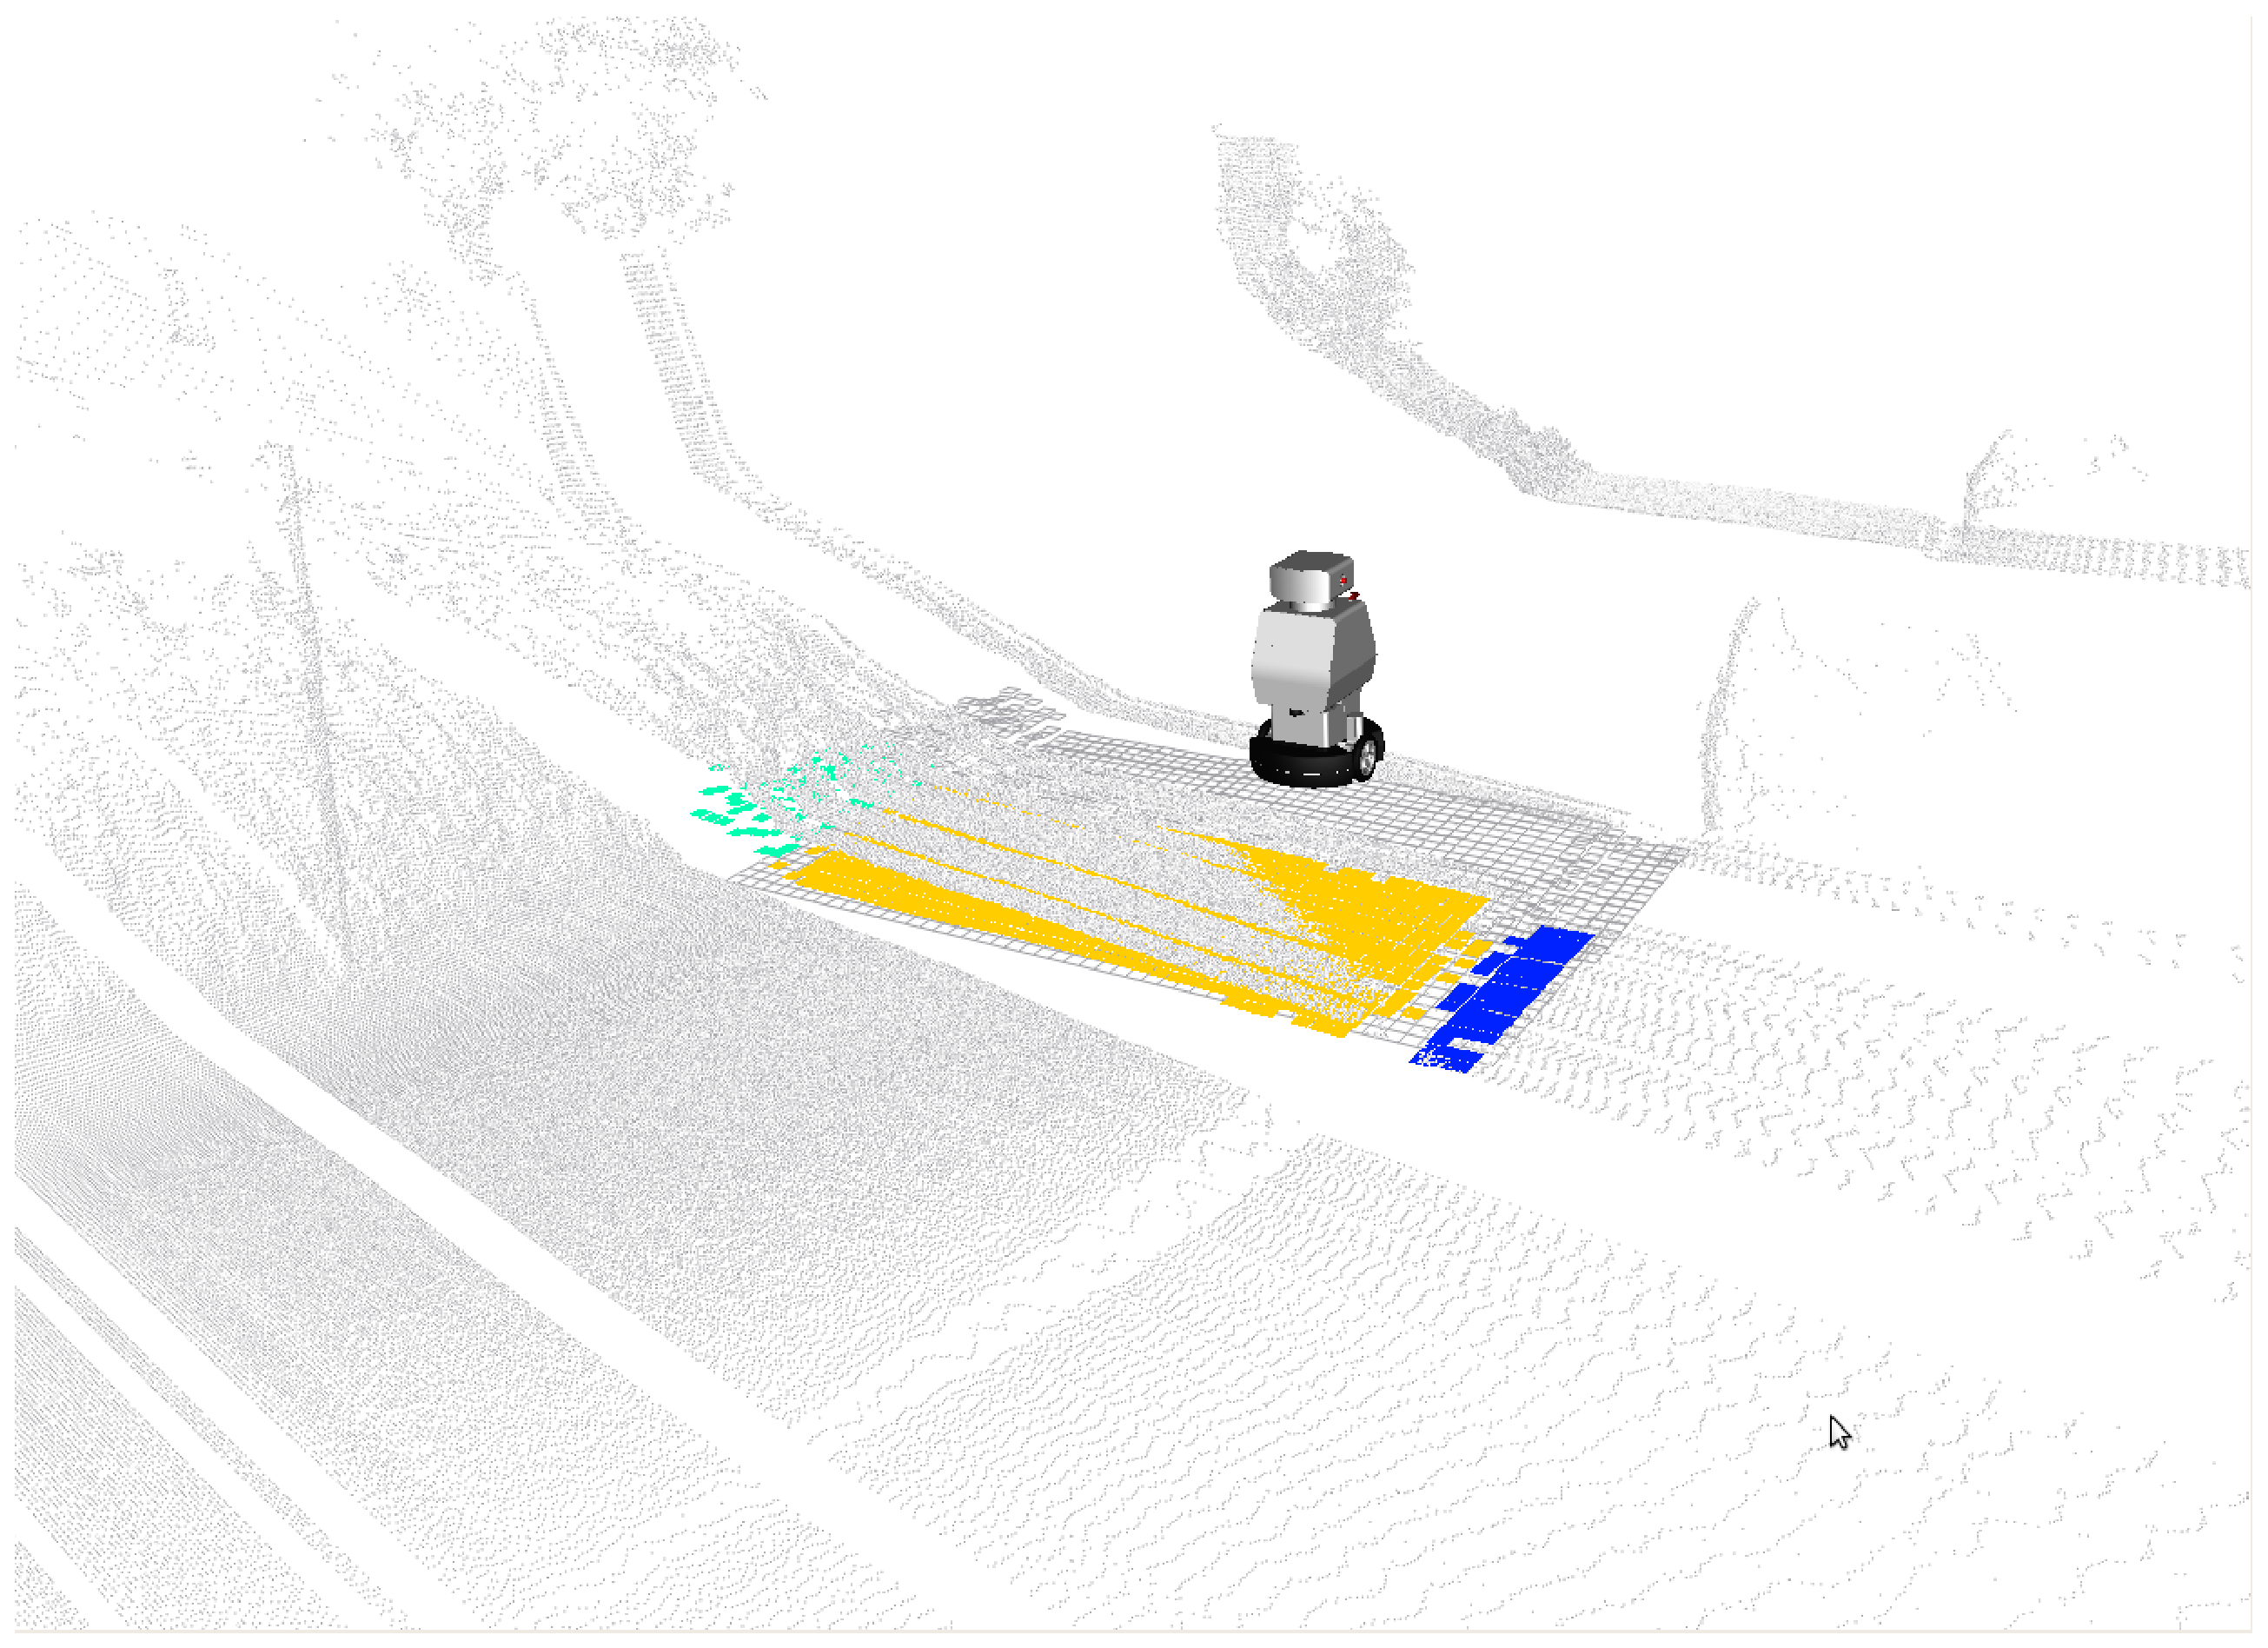
\includegraphics[width=\columnwidth]{fig/europa.eps}
\caption{Example of curb detection from a moving pedestrian robot. Colors
represent planes and curbs are located at their boundaries.}
\label{fig:europa}
\end{figure}

Fig.~\ref{fig:special} depicts a situation that a pedestrian robot might often
encounter when crossing a street. This experiment illustrates that our method
can cope with multiple viewpoints and environment configurations. Most of the
competitive approach would fail in this case.

\begin{figure}[t]
\centering
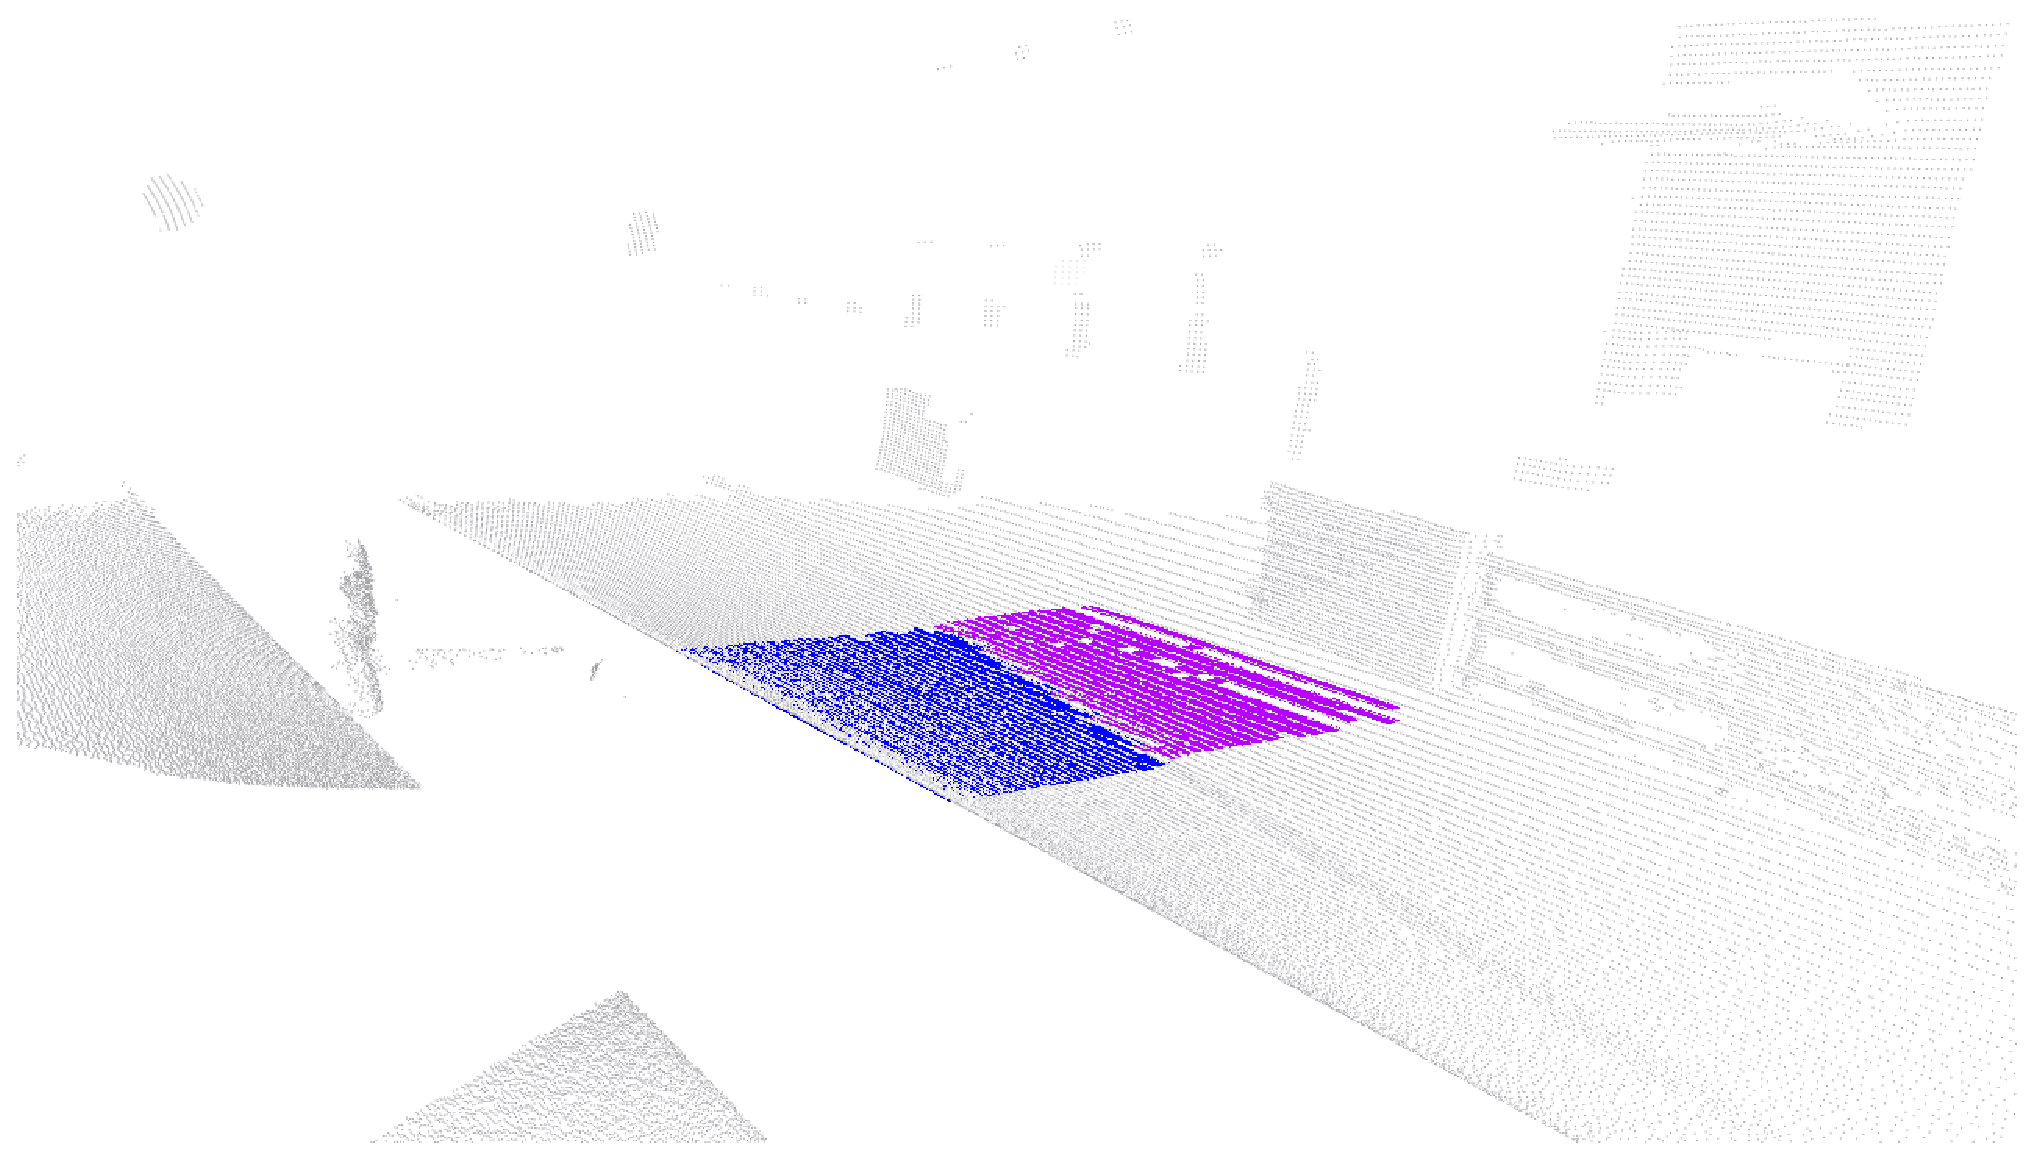
\includegraphics[width=\columnwidth]{fig/special.eps}
\caption{Example of curb detection in an unfavorable situation. Our algorithm
correctly label the planes, and thus curbs, under various viewpoints and
experimental settings.}
\label{fig:special}
\end{figure}

Fig.~\ref{fig:segment}

\subsection{Quantitative Evaluation and Discussion}



\section{Conclusion\label{sec:conc}}
In this paper, we have presented a novel approach for ...

In a further work, we aim at ...


\section*{Acknowledgment}
This work has partly been supported by the EC under FP7-231888-EUROPA.

\bibliographystyle{sty/IEEEtran}
\bibliography{bib/bibliography}

\end{document}
